\section{Computing $\BLap(\Phi)$}
In this section, we propose an Whitening-based Algorithm to compute an approximation $\BLap(\Phi)$ of backbone.

\cite{Par03} proposed an Whitening algorithm which was supposed to determine nodes that always have the same color in all legal colorings of the coloring problem.
This algorithm was also used to compute (non-)frozen literals of model clusters in SAT problem \cite{LMZ09}, from which we can compute (non-)backbone literals.


\begin{algorithm}
\SetKwInOut{Input}{Input}
\SetKwInOut{Output}{Output}
\SetAlgoShortEnd
\SetFillComment
\Input{a formula $\Phi$ and a model $\lambda$ of $\Phi$}
\Output{white clauses $W_c$ and white variables $W_v$}
$W_c:= \{\phi\in\Phi \mid \exists l_1,l_2\in\phi: \  \lambda\models l_1\wedge l_2\}$\;
$W_v:=\{x\in \var(\Phi)\mid \lambda\models x\Rightarrow x\not\in \Lit(\Psi\setminus W_c),
        \ \lambda\models \neg x\Rightarrow \neg x\not\in \Lit(\Psi\setminus W_c)\}$\;
\Repeat{No Update of $W_c$ and $W_v$}{
   $W_c := W_c \cup \{\phi\in\Phi \mid \var(\phi)\cap W_v\neq \emptyset \}$\;
   $W_v := W_v \cup \{x\in \var(\Phi)\mid \lambda\models x\Rightarrow x\not\in \Lit(\Psi\setminus W_c),
        \ \lambda\models \neg x\Rightarrow \neg x\not\in \Lit(\Psi\setminus W_c)\}$
}
\Return $(W_c, W_v)$\;
\caption{Whitening algorithm}
\label{alg:whitening}
\end{algorithm}

Given a satisfiable formula $\Phi$ and a model $\lambda$ of $\Phi$,
Algorithm \ref{alg:whitening} computes a set of white clauses $W_c$ and white variables $W_v$ by iteratively making variables and clauses as white.
The remaining non-while variables give use an under-approximation of frozen literals in the model $\lambda$ of $\Phi$, namely,
$F(\Phi,\lambda)=\Lit(\Phi)\cap \{x,\neg x\mid x\in \var(\Phi)\setminus W_v(\Phi,\lambda)\}$ is a subset of frozen literals in the model $\lambda$ of $\Phi$.


Initially, all the clauses which contain at least two satisfied literals by $\lambda$ are marked as white.
Then, each variable $x$ whose value in $\lambda$ do not satisfy any non-white clauses is marked as white.
Intuitively, if $\lambda(x)$ is $1$ and the literal $x$ does not appear in any non-white clauses $\Phi\setminus W_c$, then $x$ is marked as white. In this case,
the assignment $\lambda[\neg x]$ satisfies all the non-white clauses, because no literal
$x$ appears in them, while the assignment $\lambda[\neg x]$ also satisfies white clauses, because there are at least two literals in each of white clauses
satisfied by $\lambda$. We get that the assignment $\lambda[\neg x]$ is a model of $\Phi$ which implies that $\lambda[\neg x]\in \cl_\Phi(\lambda)$.
On the other hand, if $\lambda(x)$ is $0$ and the literal $\neg x$ does not appear in any non-white clauses $\Phi\setminus W_c$, then $x$ is marked as white.
Since the assignment $\lambda[\neg x]$ satisfies all the non-white clauses thanks to the absence of the literal
$\neg x$ in them, and satisfies all the white clauses due to fact that there are at least two literals in each of white clauses satisfied by $\lambda$.
We still get that the assignment $\lambda[\neg x]$ is a model of $\Phi$ and $\lambda[\neg x]\in \cl_\Phi(\lambda)$.
Therefore, we can infer that if the variable is $x$ white, then the literals $\neg x$ and $x$ cannot be frozen literals.

Next, Algorithm \ref{alg:whitening} iteratively and alternatively marks each clause that contain at least one white variable and each variable whose value in $\lambda$ do not satisfy any non-white clause are marked as white, until no more clause or variable can be marked as white.
This loop manages to mark as many as variables as white [possible?].
After Algorithm \ref{alg:whitening} has terminated, if a variable $x$ is non-white, i.e., $x\not\in W_v$, then there does not exist a model $\lambda'\in \cl_\Phi(\lambda)$ such that $\lambda(x)\neq \lambda(x')$. This implies that the literal $x$ (resp. $\neg x$) is a frozen literal
in the model $\lambda$ if $x\in \Lit(\Phi)$ (resp. $\neg x\in \Lit(\Phi)$).  However, it was pointed out by \cite{LMZ09} that there are cases in which
a literal $l$ is not a frozen literal, but the corresponding variable $\var(l)$ is marked as white. We refer to \cite{LMZ09} for details.



\begin{theorem}\cite{LMZ09}
\label{thm:whiten}
$F(\Phi,\lambda)\subseteq\FL(\Phi,\lambda)$.
\end{theorem}


Given a satisfiable formula $\Phi$ and a model $\lambda$ of $\Phi$, we use $W_v(\Phi,\lambda)$ (resp. $W_c(\Phi,\lambda)$) to denote the set
$W_v$ (resp. $W_c$) obtained by Algorithm \ref{alg:whitening} taking $\Phi$ and $\lambda$ as inputs.


From Proposition \ref{prop:Frozen-backbone} (i.e., $\BL(\Phi)\subseteq\FL(\Phi,\lambda)$) and Theorem \ref{thm:whiten},
we can get that literals in $F(\Phi,\lambda)$ have high probabilities to be backbone literals. However, the set $F(\Phi,\lambda)$ also contains non-backbone literals. We propose a heuristic strategy that intends to remove non-backbone literals from $F(\Phi,\lambda)$.


Our strategy is based on the observation of the relationship between $W_c(\Phi,\lambda)$ and backbone literals.
Consider the formula $\Phi=(a\vee\neg b)\wedge(b\vee\neg c)\wedge(c\vee\neg a)$ and the model $\lambda$ such that $\lambda(a)=\lambda(b)=\lambda(c)=1$. The backbone of the formula $\Phi$ is $\emptyset$, because the assignment $\lambda'$ such that $\lambda'(a)=\lambda'(b)=\lambda'(c)=0$ is also a model of $\Phi$.
However, by Algorithm \ref{alg:whitening},
$W_v(\Phi,\lambda)=\emptyset$, from which we get that $F(\Phi,\lambda)=\Lit(\Phi)$. To remove the non-backbone literals $a, \ b, \ c, \ \neg a, \ \neg b$ and  $\neg c$
from $F(\Phi,\lambda)$,  we introduce a dependency graph to characterize such literals $a, \ b, \ c, \ \neg a, \ \neg b$ and  $\neg c$ from  the given formula $\Phi$.


Given a formula $\Phi$, the \emph{dependency graph} $G_\Phi$ of $\Phi$ is a undirected graph $(V,E)$, where
$V=\Lit(\Phi)$ is a finite set of vertices, and $E\subseteq V\times V$ is a finite set of edges which is defined as follows:
for every literals $l_1,l_2\in\Lit(\Phi)$, $(l_1,l_2)\in E$ iff one of the following conditions hold:
\begin{itemize}
\item there exists a clause $\phi\in\Phi$ with $l_1,l_2\in \phi$, 
\item  $l_1=\neg l_2$,  
\item $l_1=l_2\in\Phi$ (i.e., $l_1$ is a clause in $\Phi$).
\end{itemize}

It is easy to see that if a node $l$ has a self-cycle (i.e., $l\in\Phi$), then $l$ must be a backbone literal of $\Phi$.
Figure \ref{fig:depend} depicts the dependency graph of the formula $(a\vee\neg b)\wedge(b\vee\neg c)\wedge(c\vee\neg a)$.
 \begin{figure}
    \centering
    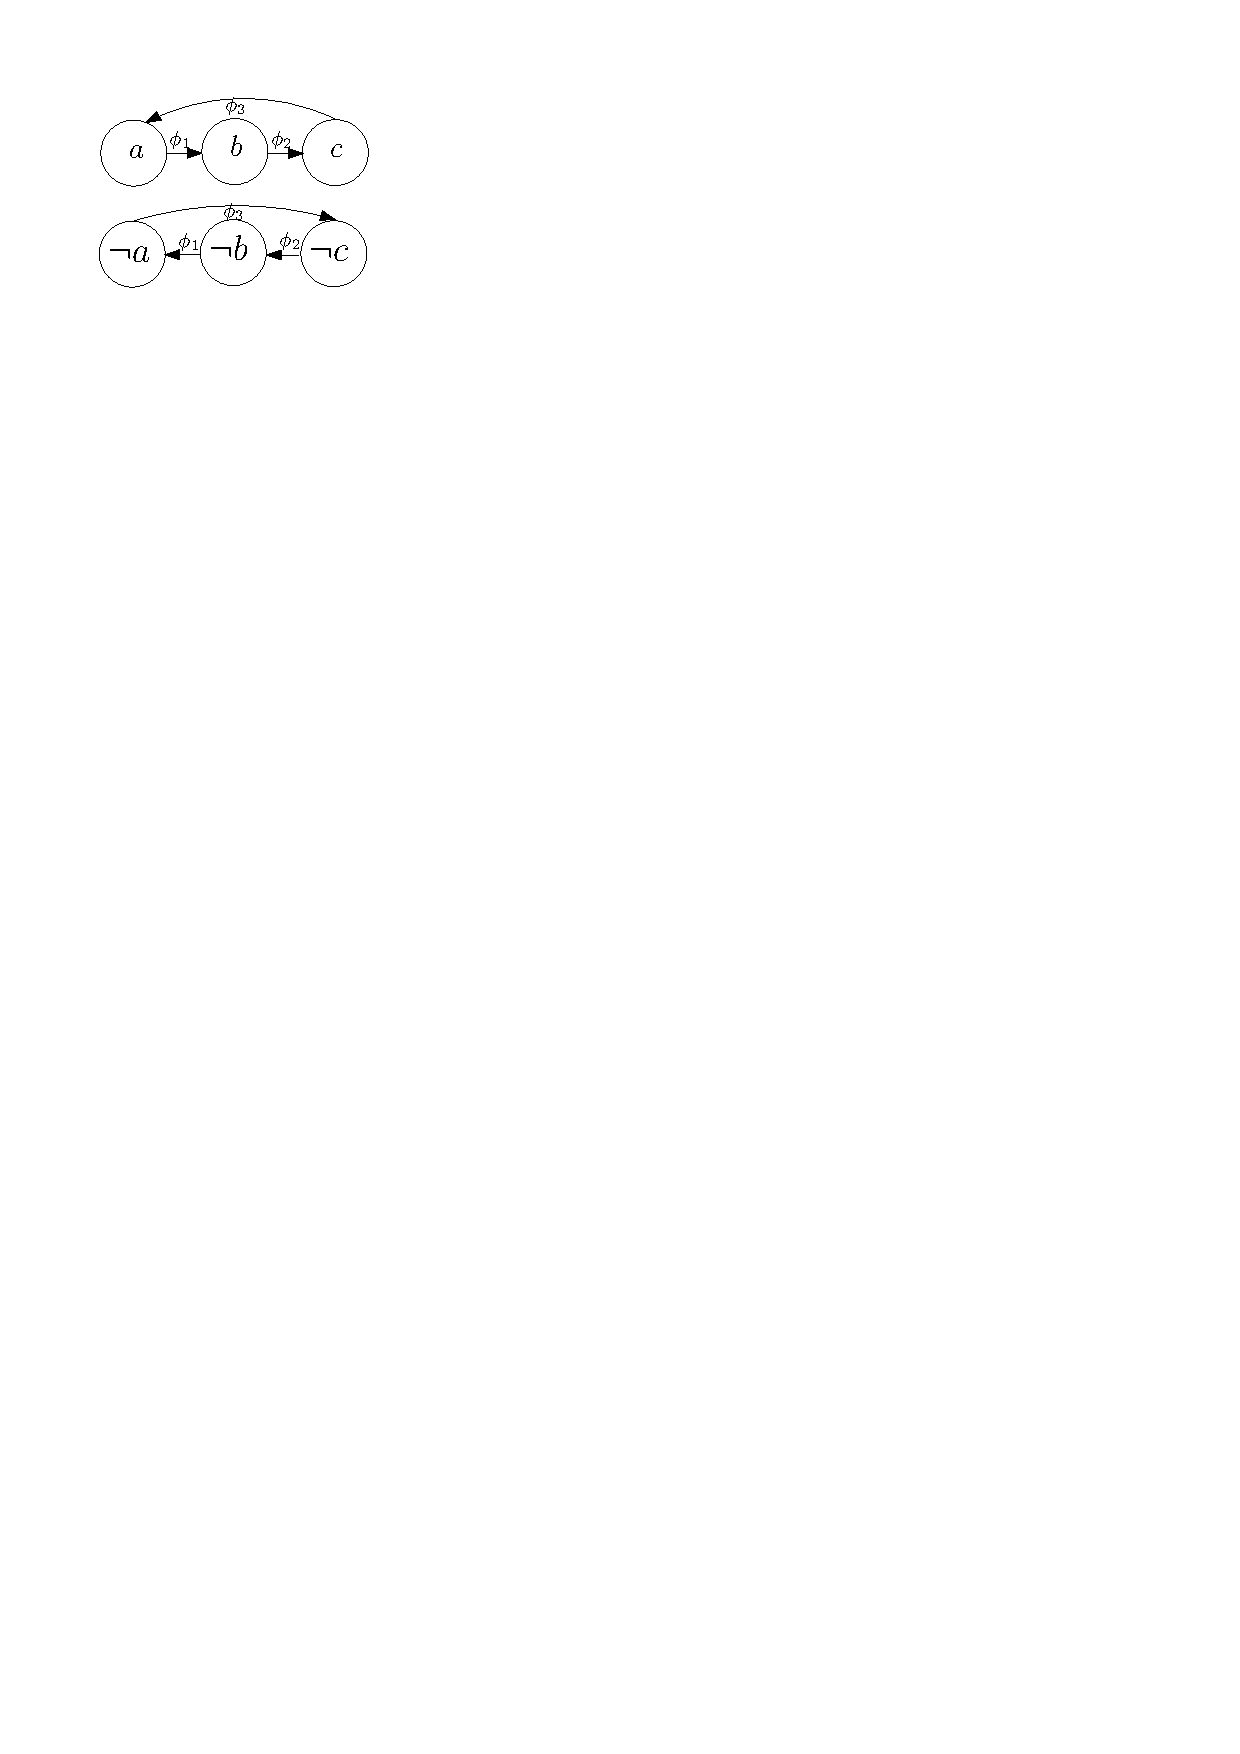
\includegraphics[scale=0.7]{dependency.pdf}
   \caption{Dependency graph of $(a\vee\neg b)\wedge(b\vee\neg c)\wedge(c\vee\neg a)$}
   \label{fig:depend}
\end{figure}

A \emph{path} $\pi$ of a dependency graph  $G_\Phi=(V,E)$ is a sequence $l_1...l_n$ of nodes, such that for every $i:\ 1\leq i<n$, $(l_i,l_{i+1})\in E$.
We use $\Lit(\pi)$ to denote the set of literals appeared in $\pi$ and $E(\pi)$ to denote the set of edges used in $\pi$.
Let $\Phi_\pi$ denote the set of clauses $\{\phi\in\Phi\mid \exists (l,l')\in E(\pi): l,l'\in \phi\}$.

A path $l_1l_2...l_n$ is \emph{valid} if $n>2$ and $|\var(\bigwedge_{1\leq i\leq n} l_i)|\geq 2$, i.e., there are at least two different variables used in
the literals  $l_1,l_2,...,l_n$. Let $\Pi(l)$ denote the set of all the valid paths starting from $l$.
A path $l_1l_2$ is \emph{trivial} if $l_1=\neg l_2$ or there exists a clause $\phi$ such that $l_1,l_2\in\phi$.
%A path $\pi=l_1...l_n$ is a \emph{pure clause path} if $l_1,...,l_n\in \Lit(\Phi_\pi)$ and $l_1,...,l_n\not\in \Lit(\Phi\setminus\Phi_\pi)$.
A valid path $l_1...l_{2n}$ is \emph{mutable} if $l_1=\neg l_{2n}$, for every $1\leq k < n$, $l_{2k}=\neg l_{2k+1}$.

\begin{proposition}
Given a model $\lambda$ of $\Phi$ and a valid mutable path $\pi$ in $G_\Phi$, 
suppose $L(\pi)=\{l_1,...,l_n\}$,  then the assignment $\lambda[\neg l_1]...[\neg l_n]$ satisfies $\Phi_\pi$.
\end{proposition}
 
 
 For every path in $\Pi(l)$, if $\Lit(\Pi(l))\setminus\{l\}$ is non-backbone literals and a new model formed when complementing every literal on the path simultaneously, then $l$ is a non-backbone literal.

 Such non-backbone checks of literals may be nested due to the dependency of literals. Therefore, instead of checking every literal in a path, we use the counterexample idea, if there exists a path $\pi$ in $\Pi(l)$, that $\Phi_{\pi}$ will be unsatisfied when complementing every literal in $\Lit(\pi)$ at the same time, then there is no immediate model from mutating a path starting from $l$.

 However, with the help of SAT solver, it's still possible to generate a model by complementing a literal that doesn't have a immediate model from mutating a path. A Mutate path just implies one possible set of literals which complementing simultaneously to generate a new model, other sets of literals are still available to generate new models.

 [Explanation]For valid paths, we want to check the possibility that complementing the literals on paths simultaneously. Given a path $\pi$, we use $\pi[i]$ to denote the $i_{th}$ literal on the path. Suppose a path with a length of four literals, $x, \neg y, y, \neg x$ respectively. It implies that $x$ and $\neg y$ are in the same clause $\phi_1$ and $y, \neg x$ are in the same clause $\phi_2$. It's obvious that both $\phi_1$ and $\phi_2$ are still satisfy by the new assignment $\lambda[\neg x, \neg y]$ from the path. The assignment $\lambda[\neg x, \neg y]$ will be a new model if $\Phi_x$ and $\Phi_y$ are either white clauses or clauses labeled in a such path. More generally, if a path with length k, contains several complementing pair of literals started from $\pi[2]$ to $\pi[k-1]$, it is refereed as \emph{mutate path}. A new assignment $\lambda[\neg l, l\in\{\pi[i] | l\in[2, k-1]\}]$ will satisfy the labeled clauses in this path. If $\Phi_l$, $l\in\{\pi[i] | l\in[2, k-1]\}$ are all white clauses or clauses labeled in a mutate path, a new model is obtained from the path.Our approach applying the counterexample idea to the facts presented above, consider a literal $l\in F(\Phi, \lambda)$ if there is a non-mutate path starting from $l$, we consider that there is no immediate model generated the literal $l$.
 However, it's possible to obtain a new model by complementing the literal that have a non-mutate path. But it's usually time-cost. In order to avoid calling SAT solvers, our approach just remove the literals that have an non-mutate path. We will apply an iteratively SAT testing Algorithm to deal with this literals.


\begin{algorithm}
\SetKwInOut{Input}{Input}
\SetKwInOut{Output}{Output}
\SetAlgoShortEnd
\SetFillComment
\Input{$\Phi$: a formula, $\NBLap$: under-approximation of non-backbone}
\Output{$\BLap(\Phi)$: backbone approximation of $\Phi$}

$\BLap:=F(\Phi, \lambda)\setminus\{l | \forall \pi, \pi[1]==l\Longrightarrow\pi[2k]==\neg\pi[2k+1], k\in[2,n-1]\}$\;
%\For{$l\in\BLap(\Phi)$}{
%    \For{$\phi\in\Phi_l$}{
%        $found:=TRUE$\;
%        $k:=1$\;
%        $\Phi_{l}^0:=\{l\}$\;
%        \Repeat {$\Phi_{l_l}^k==\Phi$}{
%            $\Phi_{l}^k:=\{\phi\in\Phi \mid \neg\Lit(\Phi_{l}^{k-1})\in\phi\}$\;
%            \If{$\neg l\in\Lit(\Phi_{l}^k)$}{
%                    break\;
%            }
%            $k++$\;
%        }
%        \If{$\Phi_{l_l}^k==\Phi$}{
%            $found:=FALSE$\;
%            break\;
%        }
%    }
%    \If{found}{
%        $\BLap(\Phi):=\BLap(\Phi)\setminus\{l\}$\;
%    }
%}
\Return $\BLap(\Phi)$\;
\caption{Backbones approximation of $\Phi$}
\label{alg:nBLo}
\end{algorithm}

Algorithm \ref{alg:nBLo} works on the dependency graph of a formula. For each literal in $F(\Phi, \lambda)$ it find all valid paths starting from the literal. If every valid path is a mutate path for the literal, then it's removed from $\BLap$. Otherwise, the literal is kept in $\BLap$ since there may not exist a model generated from complementing the literal.

Given a satisfiable formula $\Phi$, the dependency graph of $\Phi$ is $G(\Phi)$. Algorithm \ref{alg:nBLo} computes a approximation of backbone literals $\BLap$ by checking paths in $G$ started from a literal $l\in F(\Phi, \lambda)$ is a mutate path or not. If there is a not mutate path starting from literal $l$, $l$ is removed from $F(\Phi, \lambda)$.

After Algorithm \ref{alg:nBLo} has terminated, if a literal is in $F(\Phi, \lambda)$, we consider that there is a higher probability for the literal to be a backbone literal.
